\documentclass[aspectratio=169,10pt]{beamer}
\usetheme{Madrid}
\usecolortheme{default}
\usepackage{amsmath,amssymb,booktabs,graphicx,multirow,array,tikz}
\usetikzlibrary{positioning}
\usepackage[T1]{fontenc}
\usepackage{lmodern}
\graphicspath{{figures/}}
\definecolor{FullBlue}{HTML}{0072B2}
\definecolor{LagOrange}{HTML}{E69F00}
\definecolor{FaultRed}{HTML}{D55E00}
\definecolor{GoodGreen}{HTML}{009E73}
\setbeamercolor{structure}{fg=FullBlue}
\setbeamercolor{frametitle}{bg=FullBlue!10,fg=black}
\setbeamertemplate{navigation symbols}{}
\setbeamertemplate{footline}{%
  \leavevmode\hbox{%
  \begin{beamercolorbox}[wd=.62\paperwidth,ht=2.5ex,dp=1ex,leftskip=1em]{author in head/foot}%
  Real-time UWB--IMU integrity \quad Evidence: \ExecutionProfile
  \end{beamercolorbox}%
  \begin{beamercolorbox}[wd=.38\paperwidth,ht=2.5ex,dp=1ex,rightskip=1em plus1fil]{date in head/foot}%
  \hfill \insertframenumber/\inserttotalframenumber
  \end{beamercolorbox}}}
\newcommand{\ExecutionProfile}{FOCUSED\_PL}
\newcommand{\ArtifactGit}{0ed90a0d32c2}
\newcommand{\ProtocolHash}{d3d0fa4f3cd7}
\newcommand{\WeekFourStatus}{INVALID}
\newcommand{\FullATE}{0.088}
\newcommand{\LagATE}{0.088}
\newcommand{\FullPnn}{0.184}
\newcommand{\LagPnn}{0.184}
\newcommand{\FullLatency}{1.47}
\newcommand{\LagLatency}{2.40}
\newcommand{\FullNEES}{2.842}
\newcommand{\LagNEES}{2.842}
\newcommand{\PairedBlocks}{6}
\newcommand{\PairedCIUpper}{0.00}
\newcommand{\PairedVerdict}{PASS}
\newcommand{\NominalRows}{3000}
\newcommand{\RocFaultRows}{72000}
\newcommand{\FullFactors}{503}
\newcommand{\LagFactors}{401}
\newcommand{\FullOrientation}{1.710}
\newcommand{\LagOrientation}{1.710}
\newcommand{\FullConditionalAUC}{0.846}
\newcommand{\LagConditionalAUC}{0.846}
\newcommand{\PFAHolmVerdict}{FAIL}
\newcommand{\PowerNIVerdict}{PASS}
\newcommand{\IsolatedSamples}{3840}
\newcommand{\IsolatedFiniteDenominator}{2252}
\newcommand{\IsolatedContainment}{100.00}
\newcommand{\IsolatedHMI}{0}
\newcommand{\IsolatedHMIUpper}{0.078}
\newcommand{\NearBoundarySamples}{584}
\newcommand{\PersistentDetection}{98.94}
\newcommand{\PersistentMaxReject}{300}
\newcommand{\PersistentAlert}{70.72}
\newcommand{\PersistentUnavailable}{28.22}
\newcommand{\PersistentDrift}{2036.528}
\newcommand{\PersistentViolations}{0}

\title{Real-Time UWB--IMU Factor-Graph Fusion with Integrity Monitoring}
\subtitle{Architecture, Validation, and Full-History vs. Fixed-Lag Analysis}
\author{Wang Junzhe}
\date{\today}

\newcommand{\profilewarning}{%
  \begin{beamercolorbox}[sep=.45ex,center]{alerted text}
  \scriptsize \textbf{\ExecutionProfile}: complete focused PL matrices; baseline accuracy/performance/ROC remain smoke comparisons.
  \end{beamercolorbox}}
\newcommand{\full}{\textcolor{FullBlue}{full-history}}
\newcommand{\lagged}{\textcolor{LagOrange}{fixed-lag}}

\begin{document}

% 1
\begin{frame}
  \titlepage
  \vspace{-1em}
  \centering\scriptsize Artifact Git \texttt{\ArtifactGit}; report protocol \texttt{\ProtocolHash}
\end{frame}

\section{Motivation and Algorithm}
% 2
\begin{frame}{Problem statement: accuracy is not enough}
\begin{columns}[T]
\column{.54\textwidth}
\begin{block}{Navigation objective}
Estimate pose, velocity, and inertial bias at 20 Hz from 200 Hz IMU and grouped UWB ranges.
\end{block}
\begin{alertblock}{Integrity objective}
Detect a bad current range group before it contaminates the graph, and report protection levels that bound position error under the declared fault model.
\end{alertblock}
\column{.42\textwidth}
\[
\text{measurement}\rightarrow
\begin{cases}
\text{commit},&T\le\gamma\\
\text{reject},&T>\gamma
\end{cases}
\]
\vspace{.5em}
\centering Accuracy $\neq$ consistency $\neq$ integrity
\end{columns}
\end{frame}

% 3
\begin{frame}{Current development status}
\small
\begin{tabular}{p{.28\textwidth}p{.31\textwidth}p{.31\textwidth}}
\toprule
Implemented & Formally/component validated & Not yet closed \\
\midrule
Incremental iSAM2; fixed-lag marginalization; combined IMU and UWB factors; detect-before-commit; current-group PL
& Noncentral calculation; IMU MC; Method A/B shadow; 8 ROS topic scenarios; fixed-lag performance
& Week-4 Snapshot/ROC/History gates; real data; certified persistent-fault PL; FDE; multiple faults; rare-event certification \\
\bottomrule
\end{tabular}
\vspace{.8em}
\begin{alertblock}{Authoritative status}
Frozen Week-4 acceptance remains \textbf{\WeekFourStatus}. Advisor-report experiments are a separate evidence namespace and cannot change it.
\end{alertblock}
\end{frame}

% 4
\begin{frame}{End-to-end architecture}
\centering
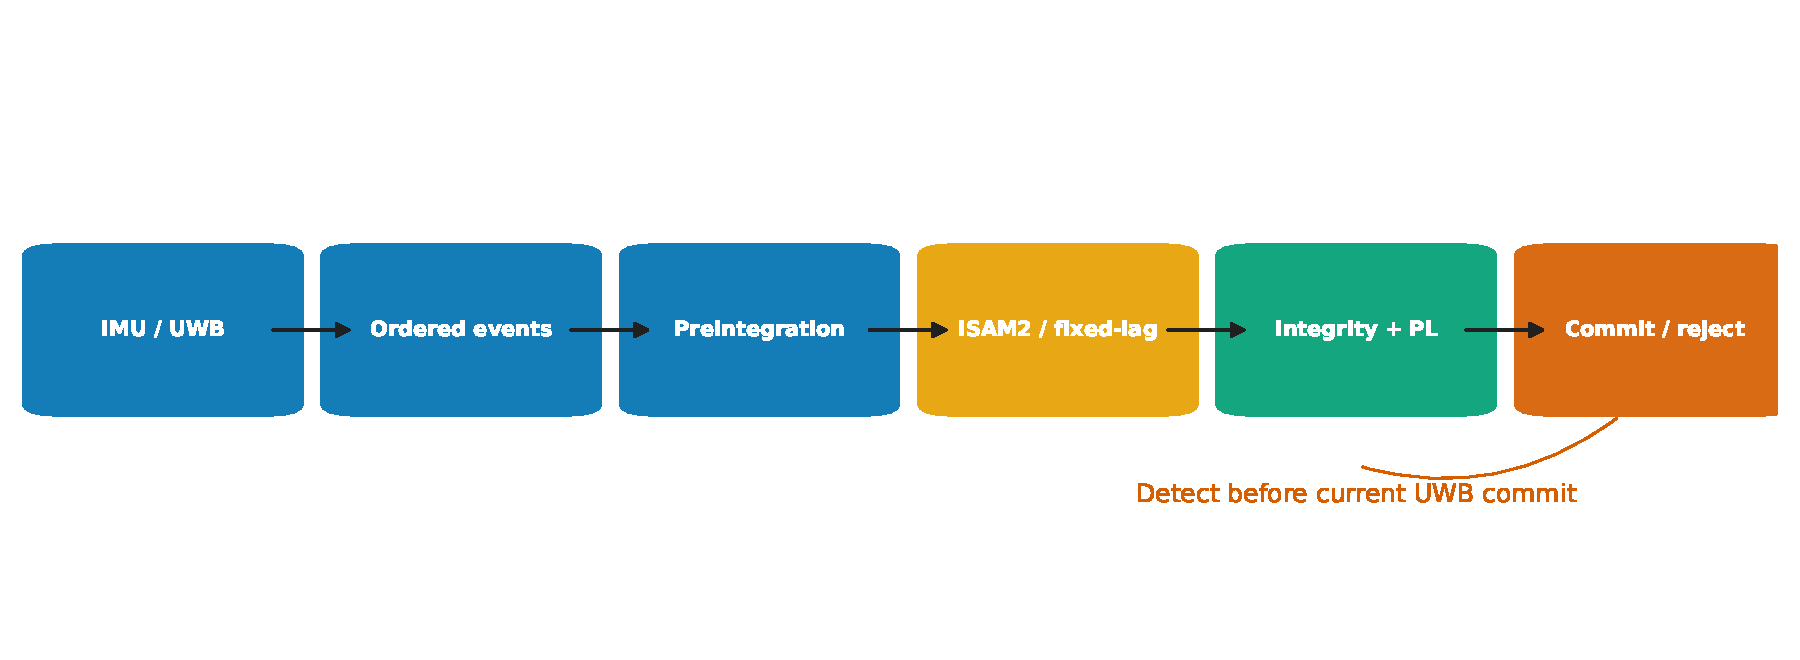
\includegraphics[width=.98\textwidth]{architecture.pdf}
\vspace{.4em}
\small Callback work is enqueue-only; one ordered worker owns state mutation and logging.
\end{frame}

% 5
\begin{frame}{State and factor graph}
\begin{columns}[T]
\column{.48\textwidth}
\[
\mathcal X_k=\{R_k,p_k,v_k,b^a_k,b^g_k\}
\]
\begin{itemize}
\item Pose prior, velocity prior, and bias prior at $k=0$.
\item Combined IMU factor links $(k-1,k)$.
\item One grouped UWB factor preserves the full range covariance.
\item iSAM2 maintains a Bayes tree; only the current clique closure is queried.
\end{itemize}
\column{.48\textwidth}
\centering
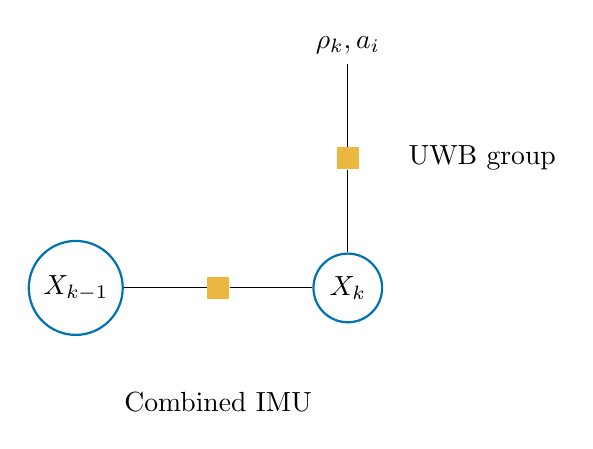
\begin{tikzpicture}[node distance=1.05cm,>=stealth]
\tikzstyle{state}=[circle,draw=FullBlue,thick,minimum size=.7cm]
\tikzstyle{factor}=[rectangle,fill=LagOrange!75,minimum size=.28cm]
\node[state] (x0) {$X_{k-1}$};
\node[factor,right=of x0] (imu) {};
\node[state,right=of imu] (x1) {$X_k$};
\node[factor,above=of x1] (uwb) {};
\node[above=of uwb] (z) {$\rho_k,a_i$};
\draw (x0)--(imu)--(x1)--(uwb)--(z);
\node[below=of imu] {Combined IMU};
\node[right=.5cm of uwb] {UWB group};
\end{tikzpicture}
\end{columns}
\end{frame}

% 6
\begin{frame}{IMU preintegration}
\small
\begin{align*}
\Delta\tilde R_{ij}&=\prod_{k=i}^{j-1}\operatorname{Exp}((\tilde\omega_k-b_i^g)\Delta t),\\
\Delta\tilde v_{ij}&=\sum_{k=i}^{j-1}\Delta\tilde R_{ik}(\tilde a_k-b_i^a)\Delta t,\\
\Delta\tilde p_{ij}&=\sum_{k=i}^{j-1}\left[\Delta\tilde v_{ik}\Delta t+\tfrac12\Delta\tilde R_{ik}(\tilde a_k-b_i^a)\Delta t^2\right].
\end{align*}
\begin{columns}
\column{.48\textwidth}
Bias correction is first order:
\[
\Delta v(b_i+\delta b)\simeq\Delta\tilde v+J_{v,b}\delta b.
\]
\column{.48\textwidth}
Error covariance propagates with the configured accelerometer, gyroscope, and bias random-walk densities.
\end{columns}
\end{frame}

% 7
\begin{frame}{UWB measurement model and provenance}
\[
r_{k,i}=\left\|p_k+R_k\ell-a_i\right\|-\rho_{k,i}
\]
\begin{itemize}
\item Physical anchor ID, world-frame coordinate, map version, measurement ID, and factor ID are retained through the integrity snapshot.
\item For grouped covariance $\Sigma_\rho=LL^\top$, rows are whitened by $L^{-1}$:
\[
e_w=L^{-1}e,\qquad H_w=L^{-1}H.
\]
\item Cholesky whitening is audited numerically; malformed or non-SPD covariance fails closed.
\item No trajectory alignment is applied when computing errors: truth and estimate already share the world frame.
\end{itemize}
\end{frame}

% 8
\begin{frame}{Two incremental backend modes}
\centering
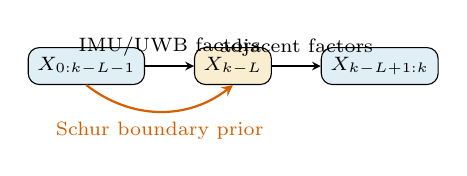
\begin{tikzpicture}[>=stealth,node distance=.62cm,every node/.style={font=\scriptsize}]
\node[draw,rounded corners,fill=FullBlue!12] (old) {$X_{0:k-L-1}$};
\node[draw,rounded corners,right=of old,fill=LagOrange!18] (boundary) {$X_{k-L}$};
\node[draw,rounded corners,right=of boundary,fill=FullBlue!12] (retained) {$X_{k-L+1:k}$};
\draw[->] (old)--node[above]{IMU/UWB factors}(boundary);
\draw[->] (boundary)--node[above]{adjacent factors}(retained);
\draw[->,FaultRed,thick,bend right=38] (old.south) to node[below]{Schur boundary prior} (boundary.south);
\end{tikzpicture}
\vspace{.3em}
\scriptsize
\begin{tabular}{p{.21\textwidth}p{.34\textwidth}p{.34\textwidth}}
\toprule
Property & \full\ incremental iSAM2 & \lagged\ incremental smoother ($L=200$)\\
\midrule
History representation & Explicit states and factors from epoch 0 & Retained window plus a Schur boundary prior\\
Relinearization scope & Affected Bayes-tree cliques; potential scope grows & Affected retained cliques and dense boundary factor\\
Graph / memory & Grows with sequence length & Bounded after the first marginalization\\
Extra work & No fixed-lag marginalization & Eliminate expired keys; update boundary prior\\
Best use & Short runs, reference solution, offline smoothing & Long-running bounded-resource navigation\\
\bottomrule
\end{tabular}
\vspace{.25em}

\small Both are incremental; ``fixed lag'' changes history representation, not the current measurement model.
\end{frame}

% 9
\begin{frame}{Detect before commit}
\centering
\Large
\textcolor{FullBlue}{predict} $\rightarrow$
\textcolor{FullBlue}{pre-UWB prior} $\rightarrow$
\textcolor{GoodGreen}{integrity test} $\rightarrow$
\textcolor{FaultRed}{commit / reject}
\vspace{1em}
\normalsize
\begin{enumerate}
\item IMU/history creates the current state key.
\item Extract $P^-$ and linearize the proposed UWB group at one consistent point.
\item Evaluate detector and protection level from a read-only snapshot.
\item Commit only if the current group passes the model and detector gates.
\end{enumerate}
\begin{alertblock}{Invariant}
The current UWB group must not appear in $P^-$; graph version, ordering version, row provenance, and pending batch ID are audited.
\end{alertblock}
\end{frame}

% 10
\begin{frame}{Conditional current-group innovation detector}
\begin{align*}
S_w &= H_wP^-H_w^\top+I,\\
T &= e_w^\top S_w^{-1}e_w \sim \chi_m^2 \quad (H_0),\\
\gamma &= F^{-1}_{\chi_m^2}(1-P_{FA}).
\end{align*}
\begin{itemize}
\item $m$ is the number of ranges in the current group; here $m=8$ nominally.
\item Global graph residual and current post-fit residual are diagnostics requiring independent empirical calibration.
\item The conditional statistic is the primary detector because its prior explicitly excludes the tested group.
\end{itemize}
\end{frame}

% 11
\begin{frame}{Protection level and declared scope}
\small
\begin{align*}
P^+ &= P^- -P^-H_w^\top S_w^{-1}H_wP^-,\\
PL_j &= K_{\rm nom}\sigma_j+\max_i g_{i,j}\sqrt{\bar\eta_i},\\
HPL&=\sqrt{PL_x^2+PL_y^2},\qquad VPL=PL_z.
\end{align*}
\begin{itemize}
\item One hypothesis per physical anchor in the current UWB group.
\item $\bar\eta_i$ comes from the noncentral $\chi^2$ missed-detection allocation.
\item Availability also requires valid geometry, valid total risk allocation, and HPL/VPL below alert limits.
\end{itemize}
\begin{alertblock}{Formal boundary}
Current-group, single-anchor range bias only. Historical persistent faults are not represented by the present fixed-lag boundary prior provenance.
\end{alertblock}
\end{frame}

\section{Experimental Design}
% 12
\begin{frame}{Research questions}
\begin{enumerate}
\item Does a 10 s fixed lag preserve full-history accuracy, covariance, and PL behavior?
\item Does fixed lag bound graph size, memory, and tail latency in practice?
\item Are conditional detector PFA, power, and time-to-detect comparable between modes?
\item Which claims are supported by deterministic simulation, and which still require formal or real-data validation?
\end{enumerate}
\end{frame}

% 13
\begin{frame}{Simulation setup}
\begin{columns}[T]
\column{.52\textwidth}
\begin{itemize}
\item Trajectories: straight, circle, figure-eight.
\item Eight 3-D anchors at cube corners $x,y=\pm5$ m, $z\in\{1,5\}$ m.
\item IMU 200 Hz; grouped UWB 20 Hz.
\item Noise and bias random walks come from the sole research YAML.
\item Same generated input object is replayed to every backend mode; digest is checked per sequence.
\end{itemize}
\column{.43\textwidth}
\begin{alertblock}{Interpretation}
High-fidelity deterministic simulation and component evidence, not measured-data validation. Errors are computed directly in the common world frame; no Umeyama alignment.
\end{alertblock}
\end{columns}
\end{frame}

% 14
\begin{frame}{Focused-PL experiment matrix}
\scriptsize
\begin{tabular}{lrrrrl}
\toprule
Suite & Modes & Seeds & Traj. & Epochs/seq. & Profile / purpose\\
\midrule
Nominal paired & 2 & 2 & 3 & 250 & smoke accuracy / NEES\\
Window ablation & 5 & 1 & 3 & 250 & smoke trade-off\\
ROC calibration/eval. & 2 & reduced & 3 & 300 & smoke detector comparison\\
Performance & 2 & 1 & 1 & 500 & smoke latency / RSS\\
Isolated fault & 2 & 640 & 3 & 312 & complete PL challenge\\
Persistent 1 m fault & 2 & 80 & 3 & 600 & complete policy invariant\\
Representative path & 2 & 1 & 1 & 1000 & complete figure-eight\\
\bottomrule
\end{tabular}
\vspace{.5em}
\begin{itemize}
\item Isolated matrix: 8 anchors $\times$ 8 fixed magnitudes $\times$ 10 seeds; seed families are disjoint.
\item Fault onset is epoch 300; only requested neighborhoods are saved, while every preceding epoch executes.
\item The two modes replay the identical generated IMU/UWB object and must share one input digest.
\end{itemize}
\profilewarning
\end{frame}

\section{Results}
% 15
\begin{frame}{Representative trajectories and anchor layout}
\centering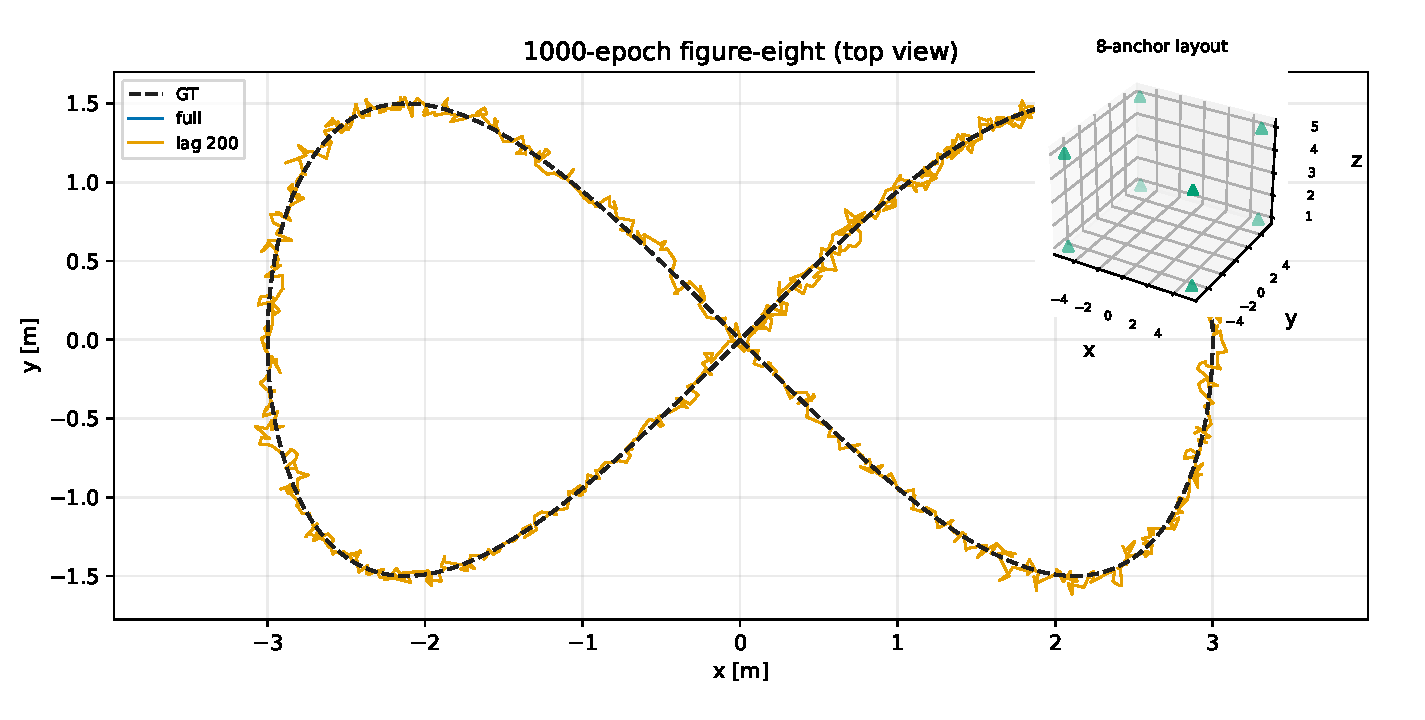
\includegraphics[width=.78\textwidth]{trajectories.pdf}
\profilewarning
\end{frame}

% 16
\begin{frame}{Nominal position accuracy}
\begin{columns}[T]
\column{.58\textwidth}
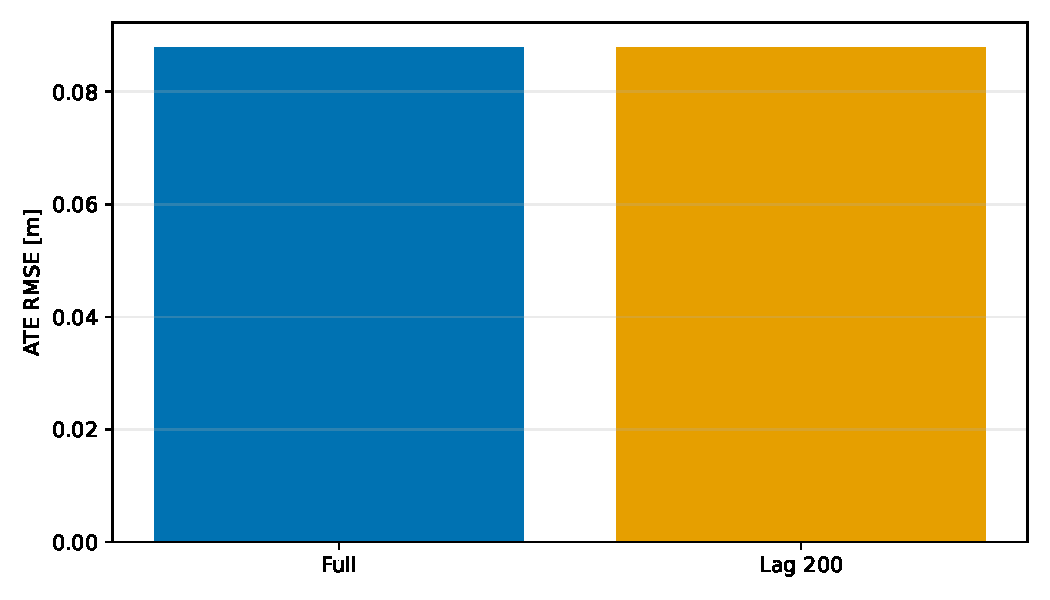
\includegraphics[width=\textwidth]{nominal_accuracy.pdf}
\column{.38\textwidth}
\small
\begin{tabular}{lcc}
\toprule & Full & Lag 200\\\midrule
ATE RMSE [m] & \FullATE & \LagATE\\
P99 [m] & \FullPnn & \LagPnn\\
Mean core [ms] & \FullLatency & \LagLatency\\
\bottomrule
\end{tabular}
\vspace{.6em}
Paired blocks: \PairedBlocks. CI upper degradation: \PairedCIUpper\%. Criterion: \PairedVerdict.
\vspace{.5em}

Current graphs contain only adjacent IMU factors and the current grouped UWB factor. Marginalizing old states transfers their information to the retained boundary through the Schur prior; therefore the current state can be numerically consistent across modes in this setup.
\end{columns}
\profilewarning
\end{frame}

% 17
\begin{frame}{Consistency and integrity containment}
\centering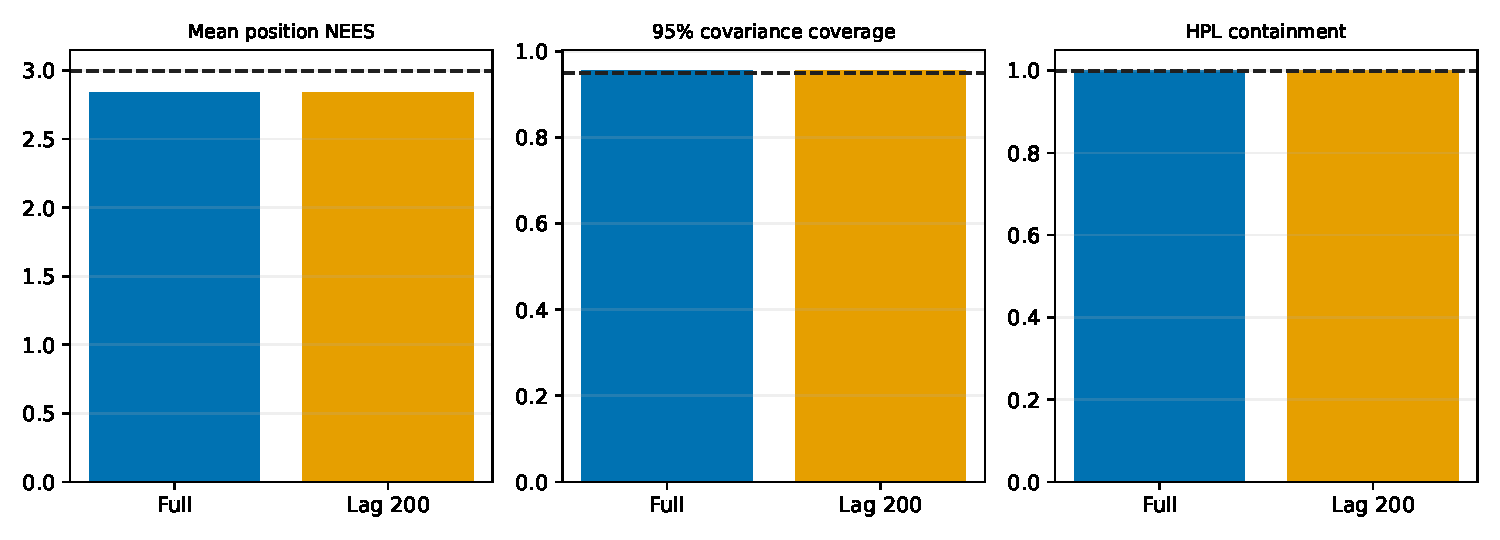
\includegraphics[width=.84\textwidth]{consistency.pdf}
\small Mean position NEES: full \FullNEES, lag \LagNEES.
\begin{alertblock}{Negative result retained}
Orientation RMSE is full \FullOrientation\ rad and lag \LagOrientation\ rad; yaw is weakly observable in this identity-attitude, range-only simulation. Position ATE must not be used to claim full navigation-state accuracy.
\end{alertblock}
\profilewarning
\end{frame}

% 18
\begin{frame}{Window-length ablation}
\centering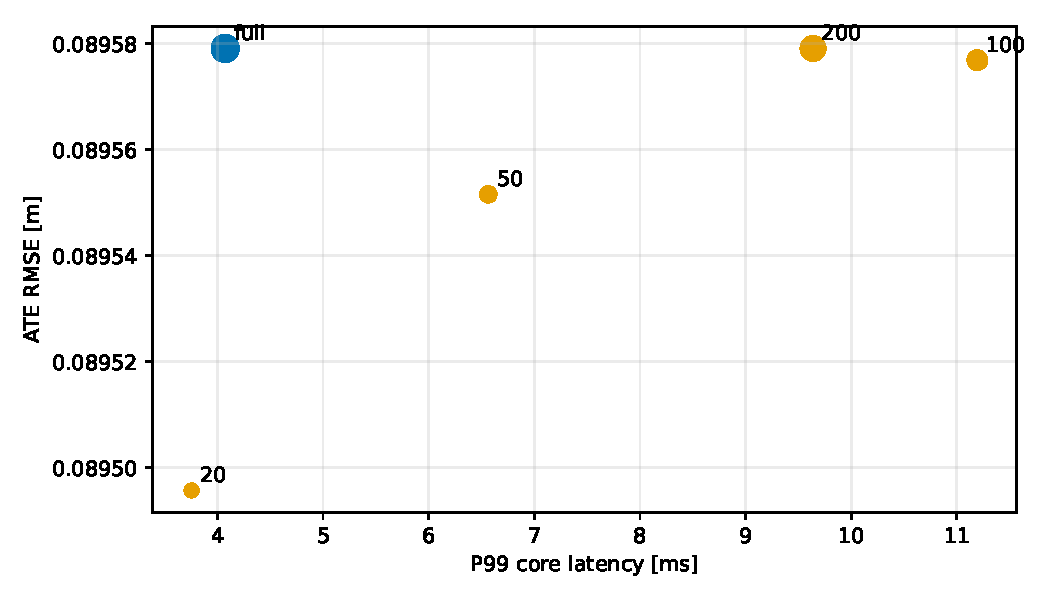
\includegraphics[height=.51\textheight]{window_ablation.pdf}
\small Marker size encodes maximum active factor count; labels are retained history lengths in epochs. A scientific trade-off is reported only after the full seed matrix is complete.
\profilewarning
\end{frame}

% 19
\begin{frame}{Latency comparison}
\centering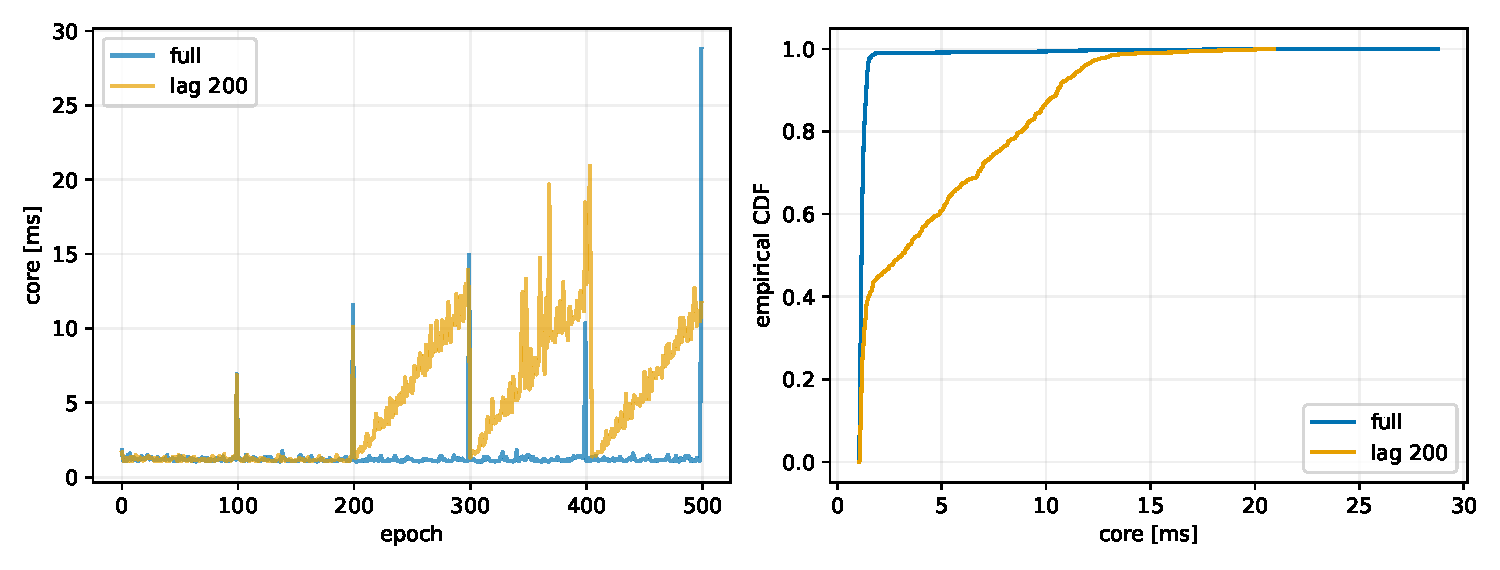
\includegraphics[width=.92\textwidth]{latency.pdf}
\small This is a 500-epoch smoke comparison. At this length the fixed-lag path pays boundary marginalization and prior-extraction cost, which can dominate any saving from a bounded graph. ``Bounded size'' does not mean ``faster at every sequence length.'' Reference lines are 50 ms mean and 100 ms P99; these data are not a platform gate.
\profilewarning
\end{frame}

% 20
\begin{frame}{Non-overlapping timing breakdown}
\centering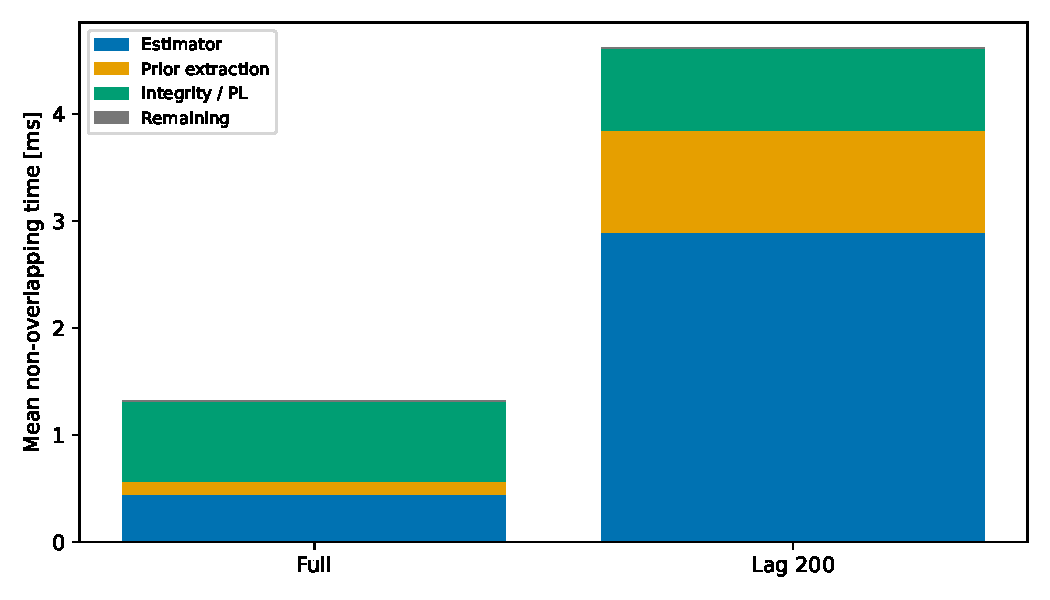
\includegraphics[height=.51\textheight]{timing_breakdown.pdf}
\small Categories partition core wall time: estimator update/commit, prior marginal and snapshot extraction, integrity/PL stages, and remaining overhead. Nested sub-timers are not summed twice.
\profilewarning
\end{frame}

% 21
\begin{frame}{Resource growth and marginalization}
\begin{columns}[T]
\column{.67\textwidth}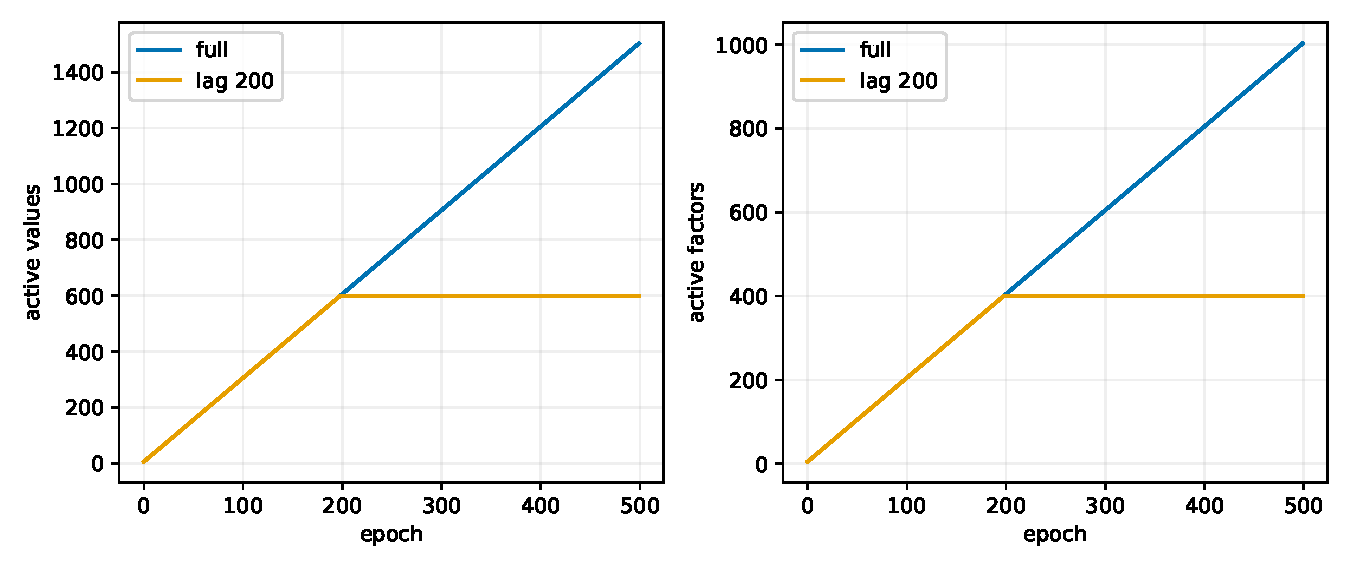
\includegraphics[width=\textwidth]{resource_growth.pdf}
\column{.29\textwidth}
\small Maximum active factors in current nominal evidence:
\begin{itemize}
\item \full: \FullFactors
\item \lagged: \LagFactors
\end{itemize}
Full-history growth is expected to continue; the 200-epoch smoother becomes bounded after marginalization begins.
\end{columns}
\profilewarning
\end{frame}

% 22
\begin{frame}{Detector ROC and AUC}
\begin{columns}[T]
\column{.64\textwidth}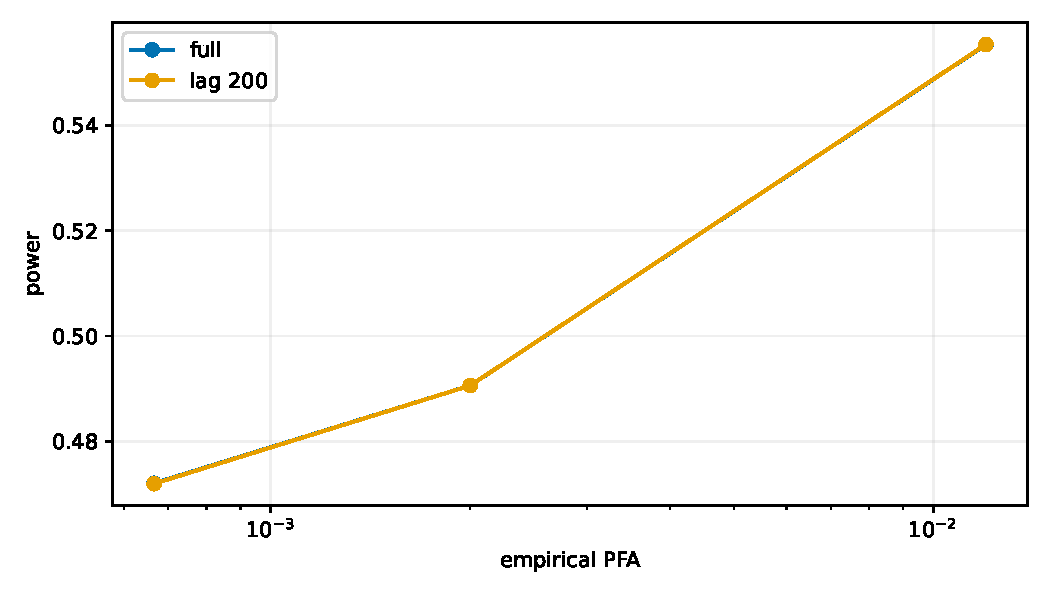
\includegraphics[width=\textwidth]{roc.pdf}
\column{.32\textwidth}
\small Conditional AUC:
\begin{itemize}
\item Full: \FullConditionalAUC
\item Lag 200: \LagConditionalAUC
\end{itemize}
Calibration, nominal evaluation, and fault seeds are disjoint. $10^{-5}$ is theory-only; finite samples cannot certify rare events.
\vspace{.5em}

Smoke Holm PFA check: \textbf{\PFAHolmVerdict}; conditional power NI check: \textbf{\PowerNIVerdict}. Both are reported, but neither upgrades the formal gate.
\end{columns}
\profilewarning
\end{frame}

% 23
\begin{frame}{Single-epoch fault: empirical PL challenge}
\centering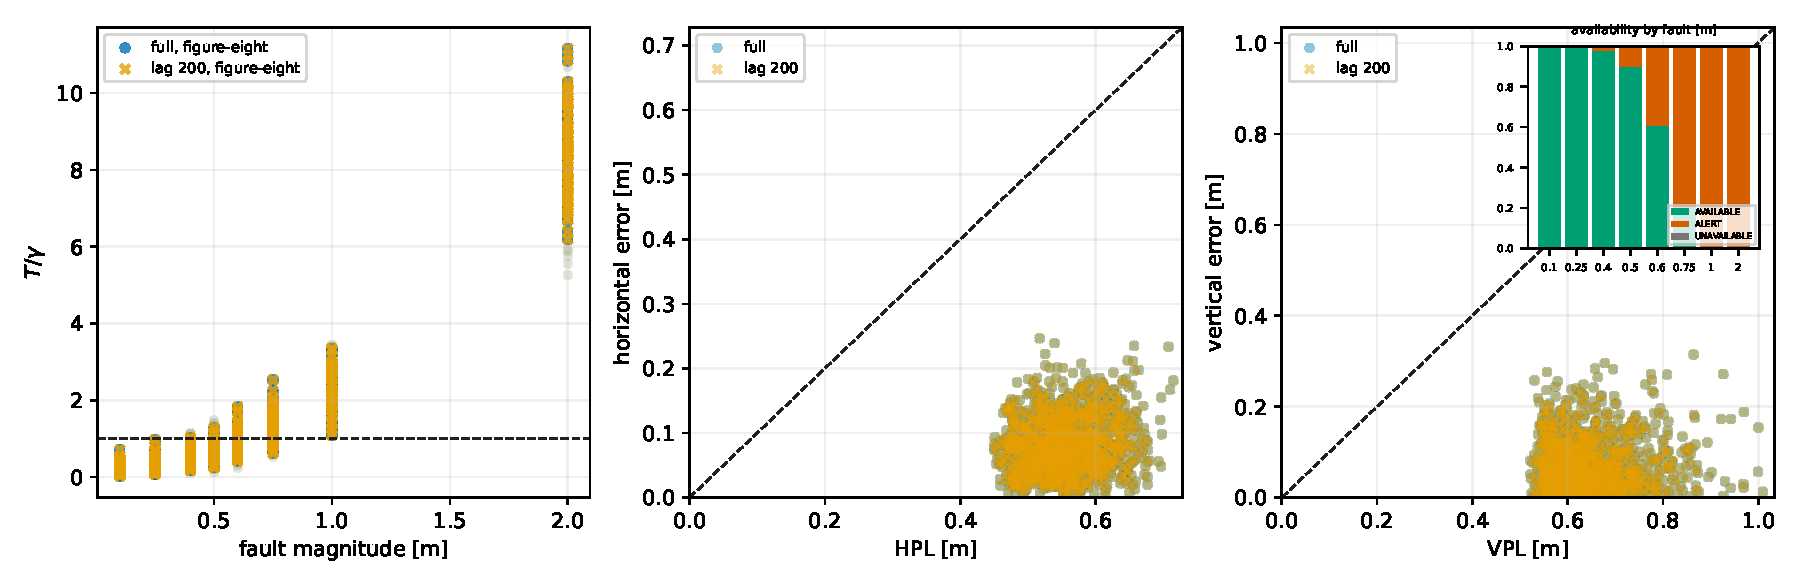
\includegraphics[width=.99\textwidth]{isolated_pl_challenge.pdf}
\scriptsize
Left: $T/\gamma>1$ is rejected. Middle/right: points below the $error=PL$ diagonal are contained; the inset reports AVAILABLE/ALERT/UNAVAILABLE fractions by magnitude. Figure-eight points are emphasized; other trajectories remain visible in pale color.

Finite-PL denominator: \IsolatedFiniteDenominator\ / \IsolatedSamples; containment: \IsolatedContainment\%; near-boundary samples ($0.8\le T/\gamma\le1.2$): \NearBoundarySamples. Observed HMI: \IsolatedHMI; one-sided exact 95\% upper rate: \IsolatedHMIUpper\%. Negative points, if any, are retained and counted.
\profilewarning
\end{frame}

% 24
\begin{frame}{Persistent 1 m fault: conservative service withdrawal}
\begin{columns}[c]
\column{.66\textwidth}\centering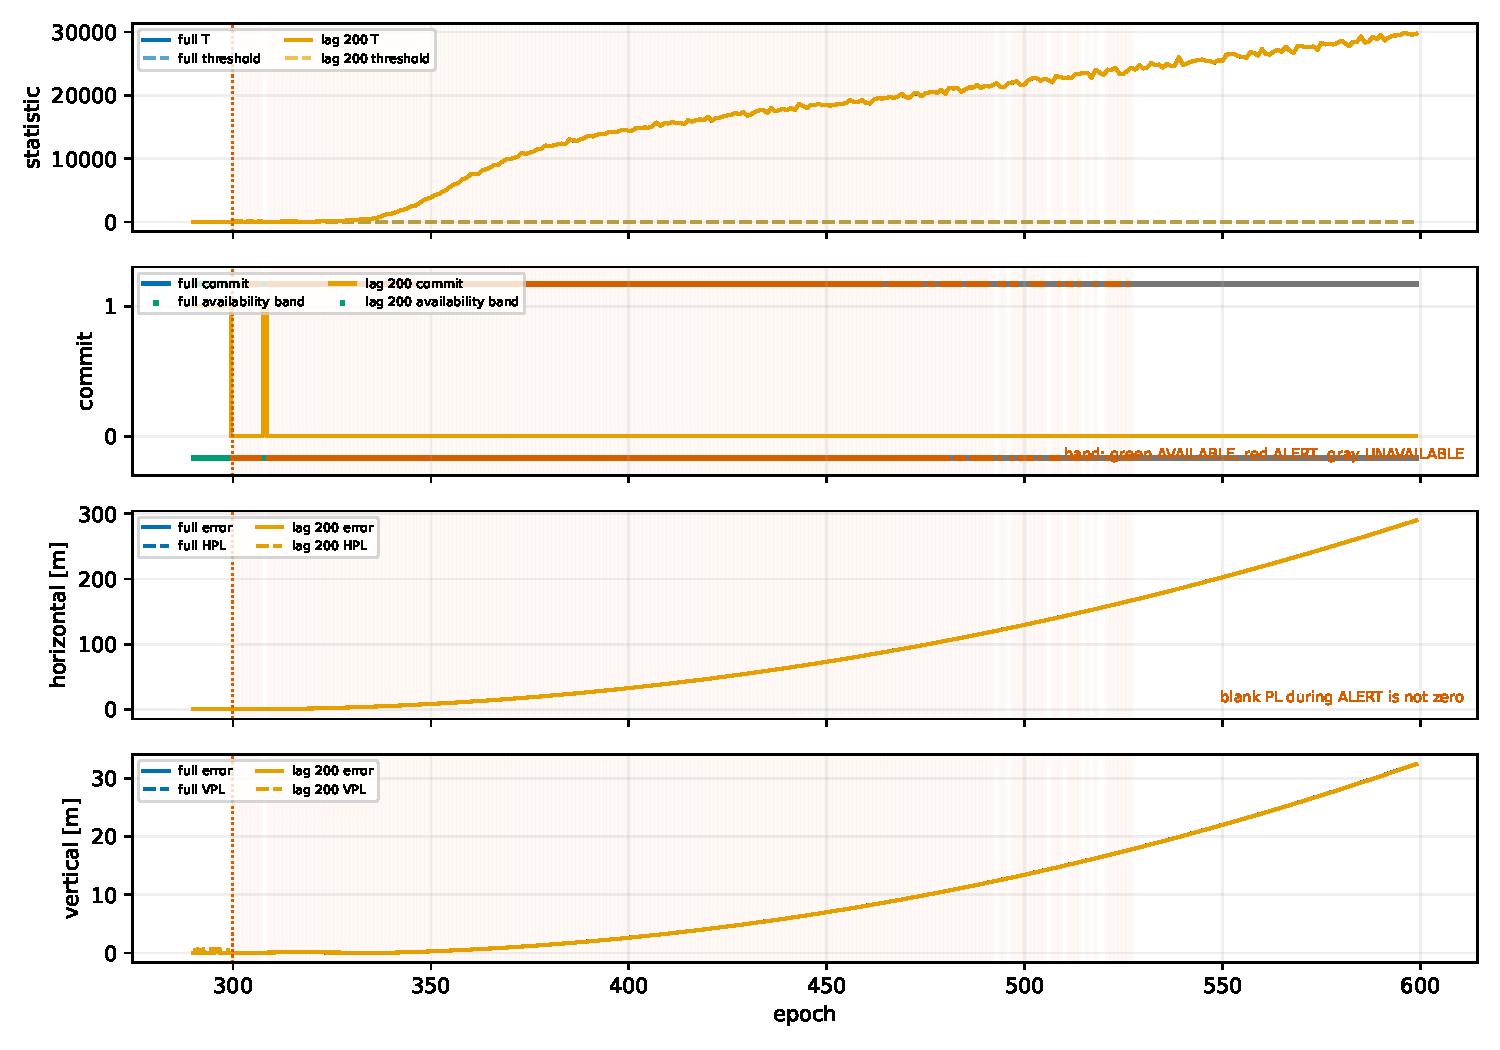
\includegraphics[height=.56\textheight]{persistent_fault_timeline.pdf}
\column{.31\textwidth}
\scriptsize
Across 8 anchors, 10 seeds/anchor, and 3 trajectories:

Rejection \PersistentDetection\%; longest run \PersistentMaxReject\ epochs; ALERT / UNAVAILABLE \PersistentAlert\% / \PersistentUnavailable\%; max IMU-only drift \PersistentDrift\ m; rejected rows with finite PL: \PersistentViolations.

Blank HPL/VPL in a red ALERT band means the integrity service was withdrawn---not zero PL and not missing plotting data.
\end{columns}
\begin{alertblock}{Claim boundary}\scriptsize
The evidence supports detection followed by integrity-service withdrawal. It is not a formal certification of PL under persistent faults.
\end{alertblock}
\profilewarning
\end{frame}

% 25
\begin{frame}{Validation dashboard: frozen evidence, not upgraded}
\centering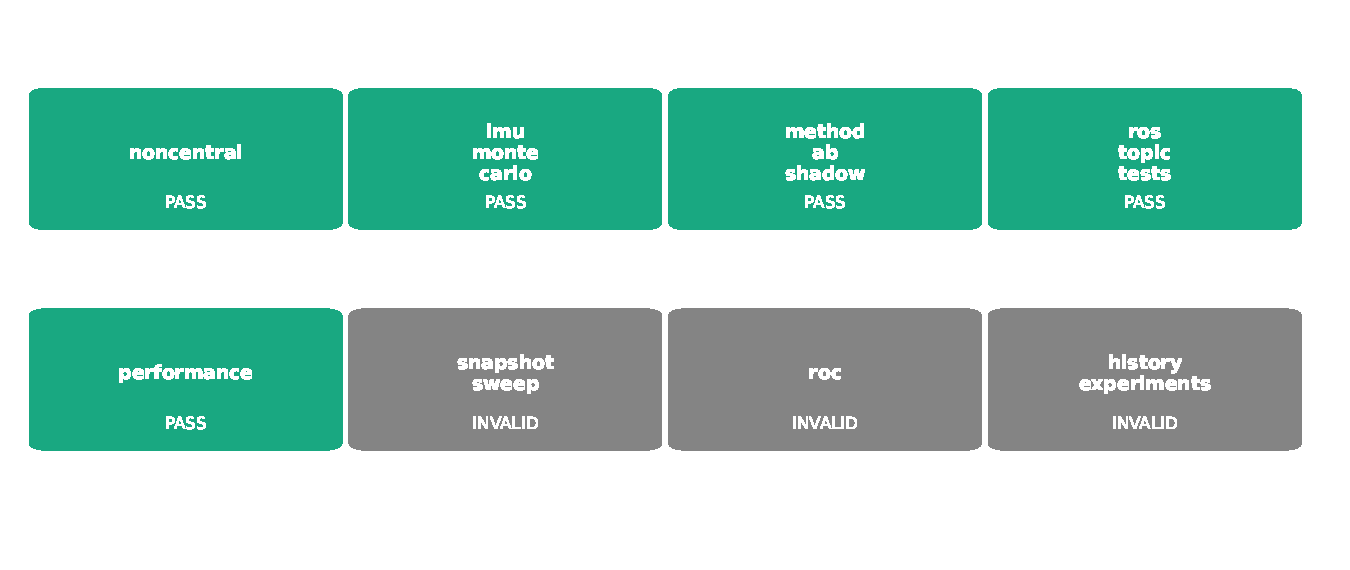
\includegraphics[width=.91\textwidth]{validation_dashboard.pdf}
\small Existing checksums were re-verified before reuse. Formal PASS: Noncentral, IMU MC, Method A/B shadow, ROS topic tests, and fixed-lag performance. Snapshot/ROC/History remain \textbf{INVALID} in frozen Week-4 acceptance.
\end{frame}

% 26
\begin{frame}{Conclusions and next steps}
\begin{block}{Supported now}
Both modes are incremental iSAM2 backends; fixed-lag uses a Schur boundary prior. The implementation enforces detect-before-commit and paired input identity. The focused challenge reports every observed HMI and confirms that rejected batches publish no finite PL.
\end{block}
\begin{alertblock}{Not supported yet}
Baseline comparisons remain smoke; orientation observability is weak; Week-4 Snapshot/ROC/History are not closed. No claim is made for real data, certified persistent-fault PL, FDE, multiple faults, TDoA, rare events, or nonlinear remainder certification.
\end{alertblock}
\textbf{Next:} add measured datasets and an outage/IMU-drift integrity model with persistent-fault provenance or FDE; then run rare-event importance sampling without changing the fixed seeds.
\end{frame}

\appendix
\section{Backup}
% 26
\begin{frame}{Backup: conditional innovation derivation}
Given $\delta x\sim\mathcal N(0,P^-)$ and $e_w=H_w\delta x+\nu_w$, $\nu_w\sim\mathcal N(0,I)$,
\[
e_w\sim\mathcal N(0,S_w),\quad S_w=H_wP^-H_w^\top+I.
\]
Let $z=S_w^{-1/2}e_w$. Under $H_0$, $z\sim\mathcal N(0,I_m)$, hence
\[
T=e_w^\top S_w^{-1}e_w=z^\top z\sim\chi_m^2.
\]
For anchor fault incidence $a_i$, the noncentrality is $\eta_i=f_i^2a_i^\top S_w^{-1}a_i$.
\end{frame}

% 27
\begin{frame}{Backup: PL ingredients and risk allocation}
\small
\begin{align*}
K &= P^-H_w^\top S_w^{-1}, & P^+ &= (I-KH_w)P^-,\\
g_{i,j} &= \frac{|e_j^\top J_pKa_i|}{\sqrt{a_i^\top S_w^{-1}a_i}}, &
P(HMI)&\le P_{NM}+\sum_i P(H_i)P_{MD,i}.
\end{align*}
The implementation checks: complete physical anchor map, monitored hypotheses, finite sensitivity, total allocated risk, current linearization version, and alert limits. Any failed prerequisite returns unavailable rather than a finite formal PL.
\end{frame}

% 28
\begin{frame}{Backup: resolved research parameters}
\scriptsize
\begin{tabular}{ll@{\qquad}ll}
\toprule
Parameter & Value & Parameter & Value\\\midrule
IMU rate & 200 Hz & UWB rate & 20 Hz\\
$\sigma_a$ & 0.10 & $\sigma_\omega$ & 0.01\\
$\sigma_{b_a}$ & 0.001 & $\sigma_{b_g}$ & 0.0001\\
Range $\sigma$ & 0.10 m & Gravity & 9.80665 m/s$^2$\\
$P_{FA}$ (formal config) & $10^{-5}$ & Total $P_{HMI}$ & $4\times10^{-5}$\\
Single-anchor $P_{MD}$ & $10^{-3}$ & Fixed lag & 200 epochs\\
HAL / VAL & 2 / 3 m & iSAM2 relin. skip & 200 updates\\
\bottomrule
\end{tabular}
\vspace{.6em}
Values are loaded from the resolved research configuration; the report protocol defines only matrices, seeds, bootstrap, and display criteria.
\end{frame}

% 29
\begin{frame}{Backup: statistical protocol}
\begin{itemize}
\item Exact timestamp matching; no spatial or temporal alignment after estimation.
\item Bootstrap unit is the full $(seed,trajectory)$ sequence, not individual epochs.
\item Calibration, nominal evaluation, and fault seed ranges are disjoint and checked.
\item PFA comparisons use Holm FWER $=0.05$ in the full campaign.
\item TTD is the first threshold crossing after the onset inside one block; undetected sequences remain censored.
\item Scientific failure is reported as FAIL. Missing, malformed, duplicate, non-finite, or incomplete artifacts are INVALID.
\end{itemize}
\end{frame}

% 30
\begin{frame}{Backup: reused component evidence}
\small
\begin{tabular}{lll}
\toprule
Component & Frozen result & Scope\\\midrule
Noncentral MC & PASS & Global bootstrap, Holm, $H_0$ checks\\
IMU MC & PASS & 3 scenarios $\times$ 100,000 trials\\
Method A/B shadow & PASS & 600/600 candidates\\
ROS topic tests & PASS & 8/8 deterministic scenarios\\
Performance & PASS & Fixed lag, 3 $\times$ 12,000 epochs\\
\bottomrule
\end{tabular}
\vspace{.8em}
Source Git and protocol hash remain those of the frozen Week-4 artifact; checksum verification succeeds. These component results do not substitute for unfinished Snapshot/ROC/History gates.
\end{frame}

% 31
\begin{frame}{Backup: Week-4 acceptance boundary}
\begin{columns}[T]
\column{.48\textwidth}
\begin{block}{PASS}
Noncentral, IMU Monte Carlo, Method A/B shadow, ROS topic tests, fixed-lag performance.
\end{block}
\column{.48\textwidth}
\begin{alertblock}{INVALID / incomplete}
Snapshot sweep, ROC, history experiments. Therefore overall status is \WeekFourStatus\ and no success token exists.
\end{alertblock}
\end{columns}
\vspace{.8em}
The advisor-report artifact records \texttt{week4\_acceptance\_modified=false}.
\end{frame}

% 32
\begin{frame}{Backup: selected references}
\footnotesize
\begin{thebibliography}{9}
\bibitem{forster} C. Forster et al., ``On-Manifold Preintegration for Real-Time Visual--Inertial Odometry,'' \emph{IEEE TRO}, 2017.
\bibitem{kaess} M. Kaess et al., ``iSAM2: Incremental Smoothing and Mapping Using the Bayes Tree,'' \emph{IJRR}, 2012.
\bibitem{fixedlag} GTSAM, Incremental Fixed-Lag Smoother documentation and implementation, version recorded in the run manifest.
\bibitem{brown} R. Brown and G. Hwang, \emph{Introduction to Random Signals and Applied Kalman Filtering}, integrity and consistency foundations.
\end{thebibliography}
\vspace{.5em}
All numerical claims in the main deck are generated from \texttt{summary.json}; no result value is hand-copied into this source.
\end{frame}

\end{document}
